% \documentclass[handout]{beamer}
\documentclass{beamer}

\mode<presentation>
{
  \usetheme{default}
  \usefonttheme[onlymath]{serif}
  % \usetheme{Singapore}
  % \usetheme{Warsaw}
  % \usetheme{Malmoe}
  % \useinnertheme{circles}
  % \useoutertheme{infolines}
  % \useinnertheme{rounded}

  \setbeamercovered{transparent=100}
}

\usepackage[english]{babel}
\usepackage[latin1]{inputenc}
\usepackage{textpos,alltt,listings,multirow,ulem,siunitx}
\usepackage{pdfpages}
\usepackage{multimedia}
\newcommand\hmmax{0}
\newcommand\bmmax{0}
\usepackage{bm}

% font definitions, try \usepackage{ae} instead of the following
% three lines if you don't like this look
\usepackage{mathptmx}
\usepackage[scaled=.90]{helvet}
% \usepackage{courier}
\usepackage[T1]{fontenc}
\usepackage{tikz}
\usetikzlibrary[shapes,shapes.arrows,arrows,shapes.misc,fit,positioning,trees,mindmap,backgrounds]

% \usepackage{pgfpages}
% \pgfpagesuselayout{4 on 1}[a4paper,landscape,border shrink=5mm]

\usepackage{JedMacros}

\title{A parallel unstructured implicit 3D polythermal model for outlet glaciers}
\author{Jed Brown,\\
Iulian Grindeanu, Dmitry Karpeev, Barry Smith, Tim Tautges}


% - Use the \inst command only if there are several affiliations.
% - Keep it simple, no one is interested in your street address.
\institute
{
  Mathematics and Computer Science Division, Argonne National Laboratory
}

\date{IGS 2012-06-28}

% This is only inserted into the PDF information catalog. Can be left
% out.
\subject{Talks}


% If you have a file called "university-logo-filename.xxx", where xxx
% is a graphic format that can be processed by latex or pdflatex,
% resp., then you can add a logo as follows:

% \pgfdeclareimage[height=0.5cm]{university-logo}{university-logo-filename}
% \logo{\pgfuseimage{university-logo}}



% Delete this, if you do not want the table of contents to pop up at
% the beginning of each subsection:
% \AtBeginSubsection[]
% {
% \begin{frame}<beamer>
%   \frametitle{Outline}
%   \tableofcontents[currentsection,currentsubsection]
% \end{frame}
% }

\AtBeginSection[]
{
  \begin{frame}<beamer>
    \frametitle{Outline}
    \tableofcontents[currentsection]
  \end{frame}
}

% If you wish to uncover everything in a step-wise fashion, uncomment
% the following command:

% \beamerdefaultoverlayspecification{<+->}

\begin{document}
\lstset{language=C}
\normalem

\begin{frame}
  \titlepage
\end{frame}

\section{Conservative models}
\begin{frame}[shrink=5]{Bathymetry and stickyness distribution}
  \begin{itemize}
  \item Bathymetry:
    \begin{itemize}
    \item Aspect ratio $\epsilon = [H]/[x] \ll 1$
    \item Need surface \emph{and} bed slopes to be small
    \end{itemize}
  \item Stickyness distribution:
    \begin{itemize}
    \item Limiting cases of plug flow versus vertical shear
    \item Stress ratio: $\lambda = [\tau_{xz}]/[\tau_{\text{membrane}}]$
    \item Discontinuous: frozen to slippery transition at ice stream margins
    \end{itemize}
  \item Standard approach in glaciology: \\
    Taylor expand in $\epsilon$ and sometimes $\lambda$, drop higher order terms.
    \begin{itemize}
    \item[$\lambda \gg 1$] Shallow Ice Approximation (SIA), no horizontal coupling
    \item[$\lambda \ll 1$] Shallow Shelf Approximation (SSA), 2D elliptic solve in map-plane
    \item Hydrostatic and various hybrids, 2D or 3D elliptic solves
    \end{itemize}
  \item \alert{\large Bed slope is discontinuous and of order 1.}
    \begin{itemize}
    \item Taylor expansions no longer valid
    \item Numerics require high resolution, subgrid parametrization, short time steps
    \item Still get low quality results in the regions of most interest.
    \end{itemize}
  \item \alert{\large Basal sliding parameters are discontinuous.}
  \end{itemize}
\end{frame}

\begin{frame}
  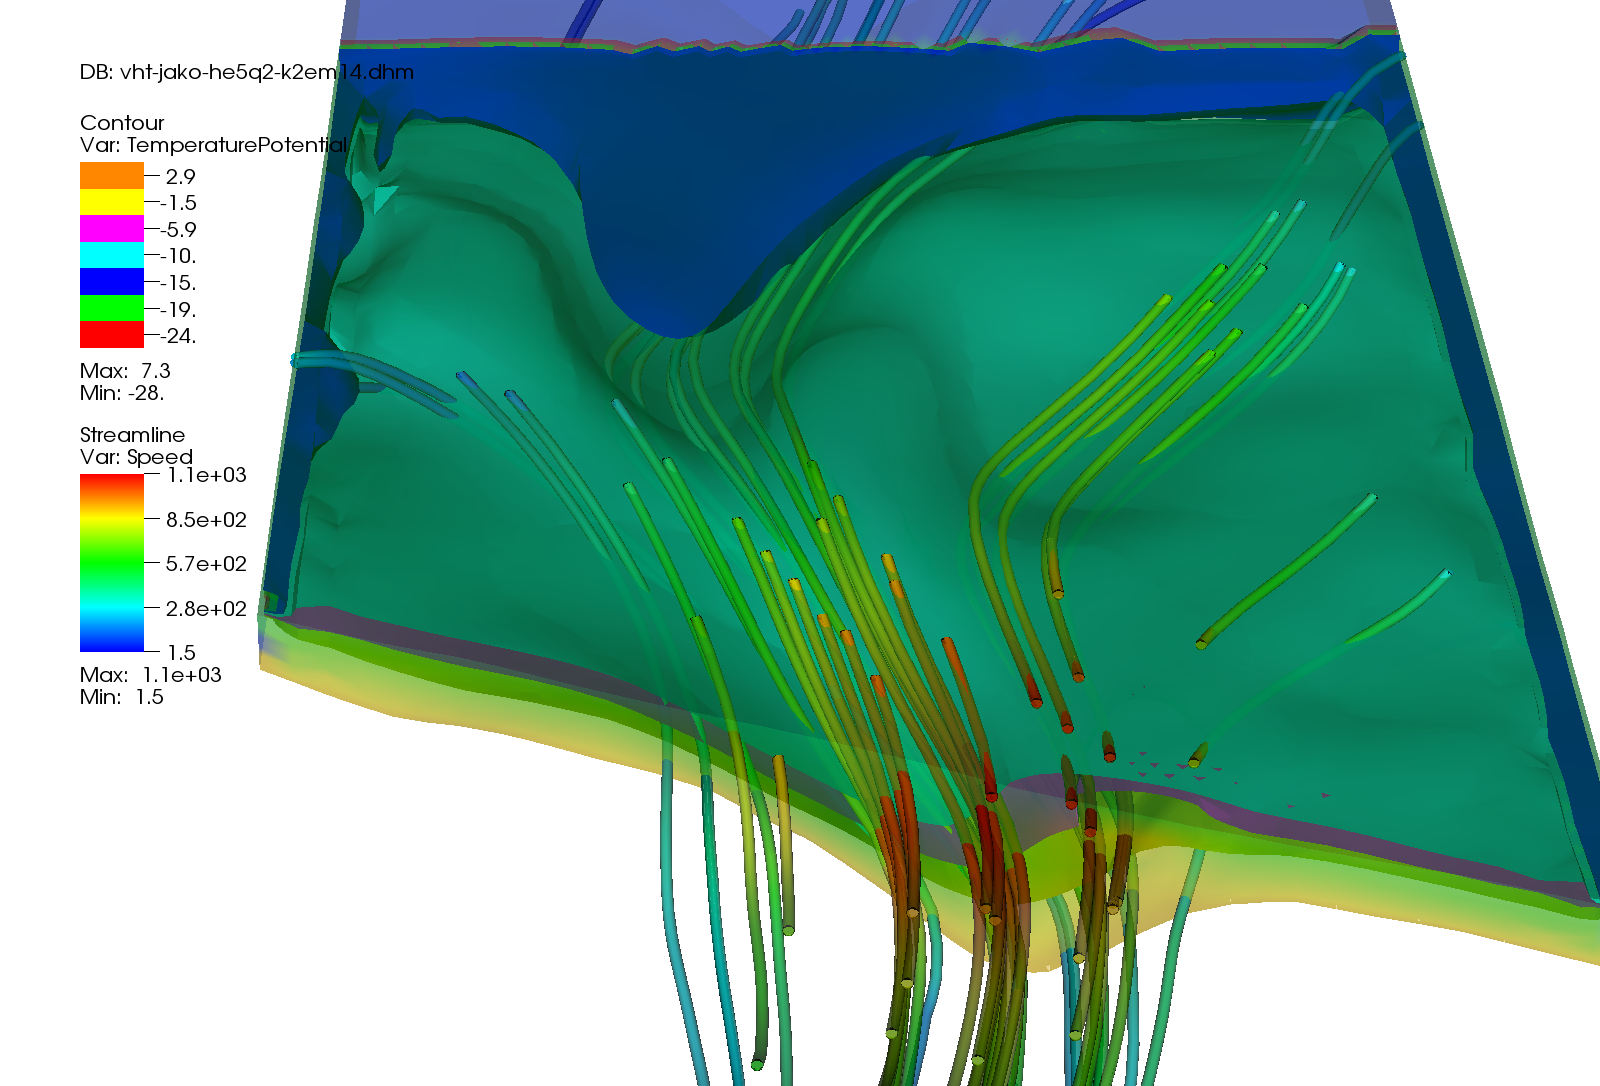
\includegraphics[width=0.8\textwidth]{figures/VHT/VHTJakoContourStream}
\end{frame}
\begin{frame}{Polythermal ice}
  \begin{itemize}
  \item Interface tracking methods (Greve's SICOPOLIS)
    \begin{itemize}
    \item Different fields for temperate and cold ice.
    \item Lagrangian or Eulerian, problems with changing topology
    \item No discrete conservation
    \end{itemize}
  \item Interface capturing
    \begin{itemize}
    \item Enthalpy: Aschwanden, Bueler, Khroulev, Blatter (J. Glac. 2012)
      \begin{itemize}
      \item Not in conservation form
      \item Only conservative for infinitesimal melt fraction
      \end{itemize}
    \item Energy
      \begin{itemize}
      \item Conserves mass, momentum, and energy for arbitrary melt fraction
      \item Implicit equation of state
      \end{itemize}
    \end{itemize}
  \end{itemize}
\end{frame}

\newcommand\smallterm[1]{{\color{gray} #1}}
\begin{frame}{Conservative (non-Boussinesq) two-phase ice flow}
  Find momentum density $\rho\uu$, pressure $p$, and total energy density $E$:
  \begin{gather*}
    (\rho\uu)_t + \div (\smallterm{\rho\uu\otimes\uu} - \eta D\uu_i + p\bm 1) - \rho \bm g = 0 \\
    \rho_t + \div \rho\uu = 0 \\
    E_t + \div \big((E+p)\uu - k_T\nabla T - k_\omega\nabla\omega \big) - \eta D\uu_i\tcolon D\uu_i - \smallterm{\rho\uu\cdot\bm g} = 0
  \end{gather*}
\begin{itemize}
\item Solve for density $\rho$, ice velocity $\uu_i$, temperature $T$, and melt fraction $\omega$ using constitutive relations.
  \begin{itemize}
  \item Simplified constitutive relations can be solved explicitly.
  \item Temperature, moisture, and strain-rate dependent rheology $\eta$.
  \item High order FEM, typically $Q_3$ momentum \& energy
  \end{itemize}
\item DAEs solved implicitly after semidiscretizing in space.
\item Preconditioning using nested fieldsplit
\item Thermomechanical steady state in about 10 nonlinear iterations
\end{itemize}
\end{frame}


\section{Conforming boundaries and model non-smoothness}
\begin{frame}{Why care about conforming and non-smoothness?}
  \begin{itemize}
  \item Subshelf ocean circulation is physically richer and more difficult to solve than ice flow
    \begin{itemize}
    \item Heat transfer is sensitive to boundary layer processes with thickness $< \SI{1}{\metre}$, $\Reynolds \sim 10^6$
    \item Countless engineering studies: wall modeling is limited, significant normal resolution still necessary
    \item Unaligned interface anisotropy is bad for Eulerian AMR methods
    \end{itemize}
  \item We care about high-dimensional sensitivity analysis and inversion
    \begin{itemize}
    \item Forward model evaluations alone are an inefficient way to explore a high-dimensional space
    \item Each source of model non-smoothness requires a lot of analysis to use adjoint methods
    \item Conforming moving mesh methods eliminate all but ``essential'' non-smoothness (like contact)
    \end{itemize}
  \end{itemize}
\end{frame}

\begin{frame}{Mesh motion via Inverse Beltrami formulation}
  \begin{itemize}
  \item nonlinear elliptic (or parabolic) equation for mesh location
  \item prescribe resolution and anisotropy using target metric tensor
  \item efficient solution using Newton-Krylov multigrid or nonlinear multigrid
  \item conservative slip boundary conditions at most surfaces
  \item ALE transport scheme corrected to satisfy geometric conservation law
  \end{itemize}
\end{frame}

\begin{frame}{Transport}
  \begin{theorem}[Godunov 1954]
    Non-oscillatory linear spatial discretizations for transport are at most first order accurate.
  \end{theorem}

  \begin{itemize}
  \item First order accurate discretizations have unacceptably high numerical diffusion
  \item Discretization choices:
    \begin{itemize}
    \item Limited or reconstructed finite volume or finite difference
      \begin{itemize}
      \item Second order TVD limiters have corners
      \item Weighted Essential Non-Oscillatory (WENO) smooth, but very nonlinear
      \item Central or upwind
      \item Inconvenient for unstructured grids
      \end{itemize}
    \item Nonlinearly stabilized continuous finite element
      \begin{itemize}
      \item Currently used, but fragile and messy
      \end{itemize}
    \item Discontinuous Galerkin
      \begin{itemize}
      \item Cell-wise entropy stability without limiters
      \item Improved robustness with smooth limiters
      \item Transitioning to this
      \end{itemize}
    \end{itemize}
  \end{itemize}
\end{frame}

\begin{frame}{}
  \begin{center}
    \color{red}{\Huge Joke}
  \end{center}
\end{frame}

\section{Multilevel Solvers}
\begin{frame}{Why do we need multilevel solvers?}
  \begin{itemize}
  \item Elliptic problems are globally coupled
  \item Without a coarse level, number of iterations proportional to inverse mesh size
  \item High-volume local communication is an inefficient way to communicate long-range information, bad for parallel models
  \item Most important with 3D flow features and/or slippery beds
  \item Nested/split multilevel methods
    \begin{itemize}
    \item Decompose problem into simpler sub-problems, use multilevel methods on each
    \item Good reuse of existing software
    \item More synchronization due to nesting, more suitable after linearization
    \end{itemize}
  \item Monolithic/coupled multilevel methods
    \begin{itemize}
    \item Better convergence and lower synchronization, but harder to get right
    \item Internal nonlinearities resolved locally
    \item More discretization-specific, less software reuse
    \end{itemize}
  \end{itemize}
\end{frame}
\begin{frame}{Relative effect of the blocks}
  \begin{equation*}\label{eq:vhtblock}
    J =
    \begin{pmatrix}
      J_{uu} & J_{up} & J_{uE} \\
      J_{pu} & 0 & 0 \\
      J_{Eu} & J_{Ep} & J_{EE}
    \end{pmatrix} .
  \end{equation*}
  \begin{itemize}
  \item[$J_{uu}$] Viscous/momentum terms, nearly symmetric, variable coefficionts, anisotropy from Newton.
  \item[$J_{up}$] Weak pressure gradient, viscosity dependence on pressure (small), gravitational contribution (pressure-induced density variation).
    Large, nearly balanced by gravitational forcing.
  \item[$J_{uE}$] Viscous dependence on energy, very nonlinear, not very large.
  \item[$J_{pu}$] Divergence (mass conservation), nearly equal to $J_{up}^T$.
  \item[$J_{Eu}$] Sensitivity of energy on momentum, mostly advective transport.
    Large in boundary layers with large thermal/moisture gradients.
  \item[$J_{Ep}$] Thermal/moisture diffusion due to pressure-melting, $\uu \cdot \nabla$.
  \item[$J_{EE}$] Advection-diffusion for energy, very nonlinear at small regularization.
    Advection-dominated except in boundary layers and stagnant ice, often balanced in vertical.
  \end{itemize}
\end{frame}

\begin{frame}{How much nesting?}
  \begin{columns}
    \begin{column}{0.5\textwidth}
      \begin{equation*}
        P_1 =
        \begin{pmatrix}
          J_{uu} & J_{up} & J_{uE} \\
          0 & B_{pp} & 0 \\
          0 & 0 & J_{EE} \\
        \end{pmatrix}
      \end{equation*}
      \begin{itemize}
      \item $B_{pp}$ is a mass matrix in the pressure space weighted by inverse of kinematic viscosity.
      \item Elman, Mihajlovi\'c, Wathen, JCP 2011 for non-dimensional isoviscous Boussinesq.
      \item Works well for non-dimensional problems on the cube, not for realistic parameters.
      \end{itemize}
    \end{column}
    \begin{column}{0.5\textwidth}
      \begin{equation*}
        P =
        \begin{bmatrix}
          \begin{pmatrix}
            J_{uu} & J_{up} \\
            J_{pu} & 0
          \end{pmatrix} & \\
          \begin{pmatrix}
            J_{Eu} & J_{Ep}
          \end{pmatrix}
          & J_{EE}
        \end{bmatrix}
      \end{equation*}
      \begin{itemize}
      \item Inexact inner solve using upper-triangular with $B_{pp}$ for Schur.
      \item Another level of nesting.
      \item GCR tolerant of inexact inner solves.
      \item Outer converges in 1 or 2 iterations.
      \end{itemize}
    \end{column}
  \end{columns}
  \begin{itemize}
  \item Low-order preconditioning full-accuracy unassembled high order operator.
  \item Build these on command line with PETSc \cverb|PCFieldSplit|.
  \end{itemize}
\end{frame}


\begin{frame}{Full Approximation Scheme}
  \begin{align*}
    \tilde u^h &\gets S^h_{\text{pre}} u^h_0 & \text{pre-smooth} \\
    L^H u^H &= I_h^H f^h + \underbrace{L^H \hat I_h^H \tilde u^h - I_h^H L^h \tilde u^h}_{\tau_h^H} & \text{solve coarse problem for $u^H$} \\
    u^h & \gets S^h_{\text{post}} \Big[ \tilde u^h + I_H^h (u^H - \hat I_h^H \tilde u^h) \Big] & \text{apply correction and post-smooth}
  \end{align*}
  \begin{itemize}
  \item Nonlinearities from spatial discretization fixed locally
  \item No assembled matrices so better floating point utilization, less memory
  \item Makes progress on all physical components at once
  \item FD and DG good, less efficient for continuous finite element methods
  \item Influence of surface evolution is low rank, no need to visit finest level on each iteration
  \end{itemize}
\end{frame}

\begin{frame}{Outlook}
  \begin{itemize}
  \item Basal hydrology model
    \begin{itemize}
    \item Need mesh-independent statistics
    \item Numerical homogenization?
    \end{itemize}
  \item True inverse and sensitivity support, but need to invert for the right thing
  \item Dynamic remeshing after large topology changes
  \item Finish FAS multigrid for full coupled system including geometry
  \item User-friendliness of process
    \begin{itemize}
    \item Currently using georeferenced initial/boundary data via GDAL
    \item But meshing process is not fully automatic
    \item Better: multiresolution database (Mark Fahnestock)
    \end{itemize}
  \end{itemize}
\end{frame}
\end{document}
